\documentclass[t,handout]{beamer}
\usepackage{verbatim}
\usepackage{xcolor}
\usepackage{multirow}
\usepackage{amssymb}
\usepackage{tikz}
\usepackage{hyperref}
\usetikzlibrary{positioning,fit}
%\usepackage{enumitem}
\usetheme{Warsaw}
\setbeamertemplate{navigation symbols}{}
\newcommand{\blue}[1]{{\color{blue} #1}}
\newcommand{\red}[1]{{\color{red} #1}}
\newcommand{\grn}[1]{{\color{green} #1}}
\newcommand{\bluRed}[2]{{\color{blue} #1}{\color{red} #2}}
\newcommand{\qtns}[0]{\begin{center} Questions? \end{center}}
\newcommand{\nl}[1]{\vspace{#1 em}}
\newcommand{\cntrImg}[2]{\begin{center}\includegraphics[scale=#2]{#1}\end{center}}
\newcommand{\defn}[1]{{\bf #1}}
\let\emptyset\varnothing
\newcommand{\SampS}[0]{$\mathcal{S}$}

\title{Math 3070, Applied Statistics}

\setlength{\abovedisplayskip}{0pt}
\setlength{\belowdisplayskip}{0pt}
\setlength{\abovedisplayshortskip}{0pt}
\setlength{\belowdisplayshortskip}{0pt}

\begin{document}
\begin{frame}[c]
    \begin{beamercolorbox}[rounded=true,wd=\textwidth,center]{title}
        \usebeamerfont{title}\inserttitle
    \end{beamercolorbox}
    \begin{center}
        Section 1\\
        \nl{0.5}
        November 6, 2019
    \end{center}
\end{frame}
\begin{frame}[c]{Lecture Outline, 11/6}
    Section 7.4
    \begin{itemize}
        \item Confidence Intervals for unknown $\sigma$
    \end{itemize}
\end{frame}


\begin{frame}{Problem}
\begin{block}{}
If $Z$ is a standard normal random variable, what is the pdf of $Z^2$?
\end{block}
\pause Letting $F(x)$ be the cdf of $X=Z^2$, for $t\geq 0$,
\begin{align*}
F(t) = P(Z^2 \leq t) 
\uncover<3->{&= P(|Z| \leq t^{1/2}) }
\uncover<4->{= 1-2\Phi(-t^{1/2})}
\end{align*}
\uncover<5->{Differentiating, we find the pdf:}
\begin{align*}
\uncover<5->{f(t) &= F'(t) = \frac{d}{dt}(1-2\Phi(-t^{1/2})) }
\uncover<6->{= -2\phi(-t^{1/2})\frac{d}{dt}(-t^{1/2}) \\}
\uncover<7->{&= t^{-1/2}\phi(t^{-1/2})}
\uncover<8->{= \frac1{\sqrt{2\pi}}t^{-1/2}e^{-t/2}}
\end{align*}
\uncover<9->{Up to a constant factor, we recognize this as the pdf of a gamma random variable, $\frac{\lambda^k}{\Gamma(k)}t^{k-1}e^{-\lambda t}$, with $k=1/2$ and $\lambda=1/2$. }
\uncover<10->{Since both are valid pdfs, the constant factors must agree; therefore,}
$$\uncover<10->{\frac1{\sqrt{2\pi}} = \frac{(1/2)^{1/2}}{\Gamma(1/2)} }
\uncover<11->{= \frac1{\sqrt2\Gamma(1/2)} }
\uncover<12->{\implies \Gamma(1/2)=\sqrt{\pi}}$$
\end{frame}

\begin{frame}{Chi-squared Distribution}
    If $Z$ is a standard normal random variable, then $Z^2$ has a so-called \textit{chi-squared} distribution with one \textit{degree of freedom}. It turns out that this is simply a gamma distribution with $k=\lambda=1/2$.
    
    \vspace{.2cm}
    The following generalization has important applications in statistical inference,:
    \begin{block}{}
    A \emph{chi-square} random variable with $\nu$ degrees of freedom is a gamma random variable with $k=\nu/2$ and $\lambda=1/2$ and has pdf
    $$f(x) = \begin{cases}\frac1{2^{\nu/2}\Gamma(\nu/2)}x^{\nu/2-1}e^{-x/2},& x\geq 0 \\ 0, & x<0\end{cases}$$
    \end{block}
    \end{frame}

\begin{frame}{Idea}
    Assume $X_1,\ldots,X_n$ are i.i.d. with $E[X_i]=\mu$ and $Var(X_i)=\sigma^2$.
    $$\frac{X_i - \mu}{\sigma}\sim N(0,1)$$
    Recall: $S^2 = \frac{1}{n-1} \sum_{i=1}^n (X_i - \overline{X})^2 $.

    We expect $\overline{X}$ and $\mu$ to be close when $n\to \infty$.

    $$\bigg( \frac{X_i - \overline{X}}{\sigma} \bigg)^2 \approx \bigg( \frac{X_i - \mu}{\sigma} \bigg)^2 \sim \chi^2_{1}$$
    More careful analysis shows that 
    $$ \sum_{i=1}^n \bigg(  \frac{ X_i - \overline{X}}{\sigma^2} \bigg)^2 = \frac{(n-1)S^2}{\sigma^2} \sim \chi^2_{n-1}$$
    \url{https://en.wikipedia.org/wiki/Cochran\%27s_theorem\#Estimation_of_variance}
    \end{frame}

\begin{frame}{Confidence Interval for Variance of Normal}
    Suppose we want to find a confidence interval for the variance $\sigma^2$ of a normal distribution based on a random sample $X_1,\dots,X_n$.
    
    \pause \vspace{.2cm}
    The statistic $(n-1)S^2/\sigma^2$ has a so-called $\chi^2$ distribution with $\nu=n-1$ degrees of freedom.
    
    \pause \begin{block}{}
    Given a random sample $X_1,\dots,X_n$ from a normal distribution with unknown mean $\mu$ and variance $\sigma^2$,
    A $100(1-\alpha)\%$ confidence interval for $\sigma^2$ is
    $$\left[\frac{(n-1)S^2}{\chi^2_{\alpha/2,n-1}}, \frac{(n-1)S^2}{\chi^2_{1-\alpha/2,n-1}}\right]$$
    where $\chi^2_{\alpha/2,n-1}$ and $\chi^2_{1-\alpha/2,n-1}$ are critical values from a \emph{$\chi^2$ distribution} with $\nu=n-1$ degrees of freedom.
    \end{block}
    \end{frame}
    
    \begin{frame}{Chi-squared distribution}
    \vspace{-1cm}
    \begin{center}
    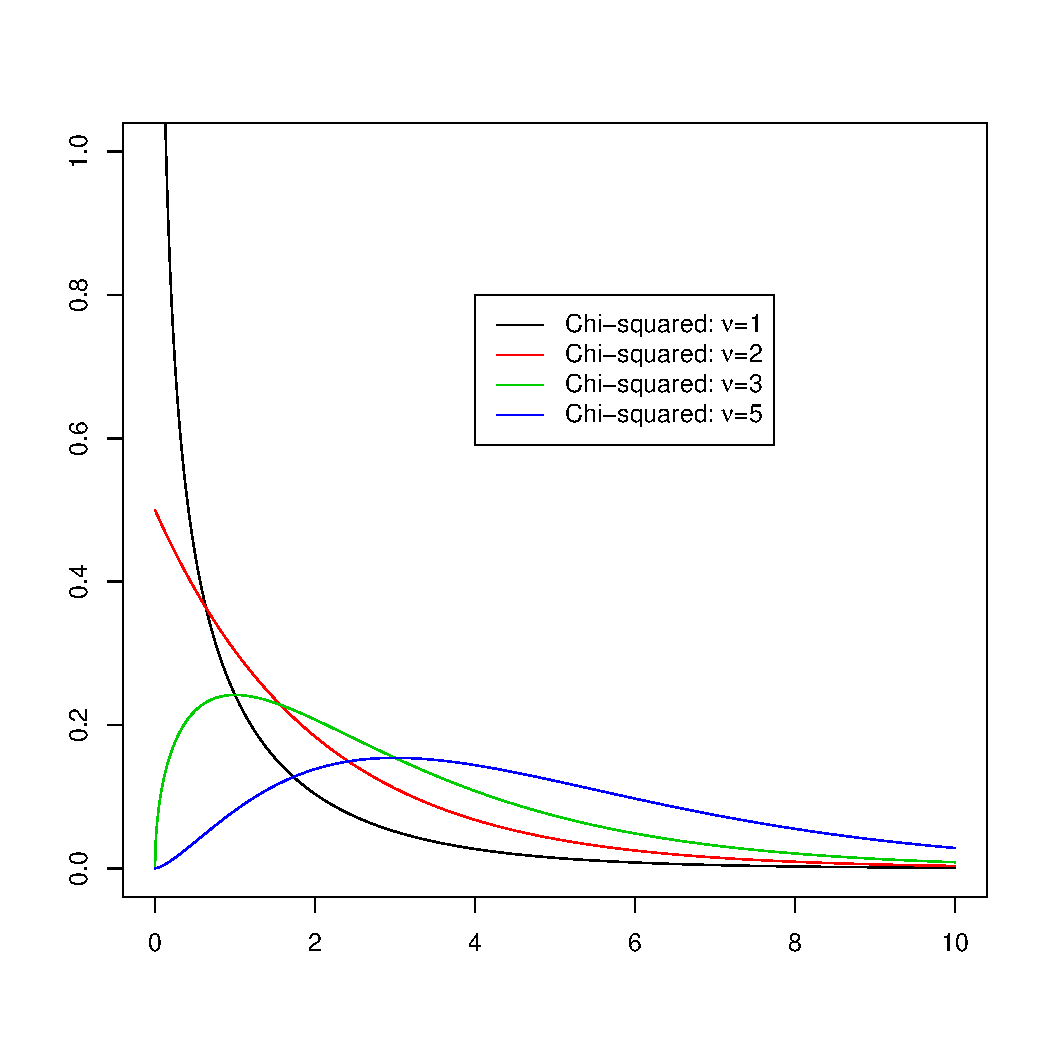
\includegraphics[scale=.5]{chisq.pdf}
    \end{center}
    \end{frame}
    
    \begin{frame}{Example}
    \begin{block}{}
    %An article reports the following data on the breakdown voltage of electrically stressed circuits, assumed to be normally distributed:
    Recall the breakdown voltage data,  assumed to be normal:
    \begin{align*}
    &1470, 1510, 1690, 1740, 1900, 2000, 2030, 2100, 2200, \\
    & 2290, 2380, 2390, 2480, 2500, 2580, 2190, 2700
    \end{align*}
    Find a 95\% confidence interval for the standard deviation $\sigma$.
    \end{block}
    
    \pause The observed sample mean and sample variance are $\overline X=2126.5$ and $S^2=137324.3$. \pause The critical values are $\chi^2_{.025,16}=28.845$ and $\chi^2_{.975,16}=6.908$, \pause which gives a 95\% confidence interval of
    $$\left[\frac{(n-1)S^2}{\chi^2_{\alpha/2,n-1}}, \frac{(n-1)S^2}{\chi^2_{1-\alpha/2,n-1}}\right]
    = [76172.3, 318064.4]$$
    for $\sigma^2$. \pause The corresponding confidence interval for $\sigma$ is
    $$[\sqrt{76172.3}, \sqrt{318064.4}] = [276.0, 564.0]$$
    % With
    %2
    %df 5 n 2 1 5 16, a 95% CI requires x2
    %.975,16 5 6.908 and x .025,16 5 28.845. The
    %interval is
    %a
    %16(137,324.3) 16(137,324.3)
    %,
    %b 5 (76,172.3, 318, 064.4)
    %28.845
    %6.908
    %Taking the square root of each endpoint yields (276.0, 564.0) as the 95% CI for s.
    
    \end{frame}
    
    
    \begin{frame}{Estimating a Proportion}
    Suppose we have a sequence of $n$ Bernoulli trials, where the probability $p$ of success is unknown. If we observe $X$ successes, we know that the maximum likelihood estimator of $p$ is the sample proportion $\hat p=X/n$. 
    
    \vspace{.2cm}\pause How do we construct a confidence interval for $p$ based on $\hat p$?
    \pause \begin{block}{}Suppose $X$ is a binomial random variable counting the number of successes in $n$ trials where each trial has probability $p$ of success. If $n$ is sufficiently large an approximate $100(1-\alpha)\%$ confidence interval is given by
    $$\hat p \pm z_{\alpha/2}\sqrt{\frac{\hat p(1-\hat p)}n}$$
    where $\hat p=X/n$ is the sample proportion, and $z_{\alpha/2}$ is a critical value from the standard normal distribution.
    \end{block}
    \pause Rule of thumb: This may be used if the number of successes $X$ and the number of failures $n-X$ are both at least 10.
    %The sample proportion $\hat p$ has mean $p$ and variance
    %$$V(\hat p) = V\left(\frac X n\right) = \frac1{n^2}V(X) = \frac1{n^2}\cdot np(1-p) = \frac{p(1-p)}n$$
    %\begin{block}{}
    %\end{block}
    %\begin{align*}
    %S^2 &= \frac1{n-1}(\sum_{i=1}^n {X_i^2}-n\overline{X}^2) \\
    %&= \frac1{n-1}(n\hat p-n\hat p^2)
    %\end{align*}
    \end{frame}
    
    \begin{frame}{Example}
    \begin{block}{}
    A quality control team for a manufacturer tests 200 randomly selected devices, out of which 15 are defective. Assume that defective devices occur independently of one another. Find an approximate 95\% confidence interval for the proportion defective.
    \end{block}
    \pause Here the sample proportion is $\hat p=15/200=.075$, and the critical value is $z_{.025}=1.96$, so the approximate 95\% confidence interval is
    \begin{align*}
    \hat p \pm z_{\alpha/2}\sqrt{\frac{\hat p(1-\hat p)}n} &= .075 \pm 1.96\sqrt{\frac{.075(1-.075)}{200}} \\
    &= .075 \pm .037
    \end{align*}
    \end{frame}
    
    \begin{frame}{Necessary Sample Size for Estimating Proportion}
    \begin{block}{}
    In the previous example, a $95\%$ confidence interval for the proportion was $.075 \pm .037$. Estimate the required sample size to achieve a margin of error of .01.
    \end{block}
    \pause Setting the margin of error equal to .01 gives an equation
    $$.01=z_{\alpha/2}\sqrt{\frac{\hat p(1-\hat p)}n}$$
    \pause Solving for $n$ gives
    $$n=\frac{z_{\alpha/2}^2\hat p(1-\hat p)}{.01^2}$$
    \pause Unfortunately, this depends on $\hat p$, which is unknown until \textit{after} the new sample is taken. \pause However, we can estimate the required $n$ by using our previous sample proportion $\hat p = .075$:
    \pause
    $$n \approx \frac{1.96^2(.075)(1-.075)}{.01^2}=2665.11 \approx 2666$$
    \end{frame}
    
    
    
    
    \begin{frame}{Summary}
    \begin{center}
    \small
    \renewcommand*{\arraystretch}{1.5}
    \begin{tabular}{p{4.5cm}|p{4cm}}
    Confidence interval for mean $\mu$ of normal, $\sigma$ known & 
    \vspace{-.25cm}$\displaystyle\overline X \pm \frac{z_{\alpha/2}\cdot\sigma}{\sqrt n}$ \\ \hline
    Large-sample approximate confidence interval for mean $\mu$ & 
    \vspace{-.25cm}$\displaystyle\overline{X} \pm \frac{z_{\alpha/2}\cdot S}{\sqrt{n}}$ \\ \hline
    Confidence interval for mean $\mu$ of normal, $\sigma$ unknown & \vspace{-.25cm}$\displaystyle\overline{X} \pm \frac{t_{\alpha/2,n-1}\cdot S}{\sqrt{n}}$ \\ \hline
    Prediction interval for normal observation & 
    \vspace{-.25cm}$\displaystyle\overline X \pm t_{\alpha/2,n-1}\cdot S\sqrt{1+\frac1n}$ \\ \hline
    Confidence interval for variance $\sigma^2$ of normal &
    \vspace{-.35cm}$\displaystyle\left[\frac{(n-1)S^2}{\chi^2_{\alpha/2,n-1}}, \frac{(n-1)S^2}{\chi^2_{1-\alpha/2,n-1}}\right]$ \\ \hline
    %Confidence interval for mean $\mu$ of exponential & 
    %\vspace{-.35cm}$\displaystyle\left[\frac{2\sum_{i=1}^n X_i}{\chi^2_{\alpha/2,2n}} ,\frac{2\sum_{i=1}^n X_i}{\chi^2_{1-\alpha/2,2n}}\right]$ \\ \hline
    Approximate confidence interval for proportion $p$ &
    \vspace{-.3cm}$\displaystyle\hat p \pm z_{\alpha/2}\sqrt{\frac{\hat p(1-\hat p)}n}$
    \end{tabular}
    \end{center}
    \end{frame}

\end{document}